% Diagrama: Bloques semánticos como modalidades del paciente
\begin{figure}[H]
\centering
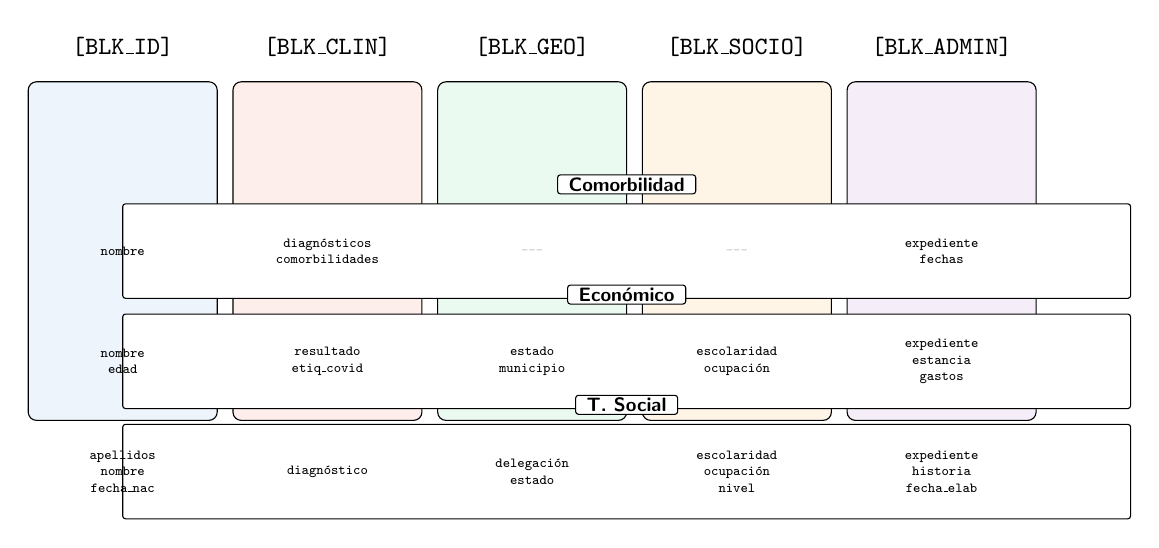
\begin{tikzpicture}[
    cell/.style={align=center, font=\tiny\ttfamily},
    rowbox/.style={draw, rounded corners=1pt, fill=white, inner sep=5pt},
    bloc/.style={draw, rounded corners=3pt, inner sep=2pt},
    rowlabel/.style={anchor=east, font=\footnotesize\sffamily},
    tab/.style={draw, rounded corners=1pt, fill=white, inner xsep=4pt, inner ysep=1pt, font=\scriptsize\sffamily\bfseries}]

\definecolor{cID}{HTML}{4A90D9}
\definecolor{cCLIN}{HTML}{E74C3C}
\definecolor{cGEO}{HTML}{2ECC71}
\definecolor{cSOCIO}{HTML}{F39C12}
\definecolor{cADMIN}{HTML}{9B59B6}

\pgfmathsetmacro{\cw}{2.4}
\pgfmathsetmacro{\cs}{0.2}
\pgfmathsetmacro{\rh}{1.2}
\pgfmathsetmacro{\rs}{0.2}

\pgfmathsetmacro{\xA}{0}
\pgfmathsetmacro{\xB}{\cw+\cs}
\pgfmathsetmacro{\xC}{2*(\cw+\cs)}
\pgfmathsetmacro{\xD}{3*(\cw+\cs)}
\pgfmathsetmacro{\xE}{4*(\cw+\cs)}
\pgfmathsetmacro{\tw}{5*\cw+4*\cs}
\pgfmathsetmacro{\bw}{\cw}
\pgfmathsetmacro{\bh}{3*\rh+2*\rs+0.3}

\pgfmathsetmacro{\yA}{0}
\pgfmathsetmacro{\yB}{-\rh-\rs}
\pgfmathsetmacro{\yC}{-2*\rh-2*\rs}

% BARRAS VERTICALES (bloques)
\node[bloc, fill=cID!10,   minimum width=\bw*1cm, minimum height=\bh*1cm] at (\xA*1cm, 0) {};
\node[bloc, fill=cCLIN!10, minimum width=\bw*1cm, minimum height=\bh*1cm] at (\xB*1cm, 0) {};
\node[bloc, fill=cGEO!10,  minimum width=\bw*1cm, minimum height=\bh*1cm] at (\xC*1cm, 0) {};
\node[bloc, fill=cSOCIO!10,minimum width=\bw*1cm, minimum height=\bh*1cm] at (\xD*1cm, 0) {};
\node[bloc, fill=cADMIN!10,minimum width=\bw*1cm, minimum height=\bh*1cm] at (\xE*1cm, 0) {};

% Etiquetas de bloques (arriba)
\node[above=2mm, font=\small\ttfamily\bfseries] at (\xA*1cm, 0.5*\bh*1cm) {\texttt{[BLK\_ID]}};
\node[above=2mm, font=\small\ttfamily\bfseries] at (\xB*1cm, 0.5*\bh*1cm) {\texttt{[BLK\_CLIN]}};
\node[above=2mm, font=\small\ttfamily\bfseries] at (\xC*1cm, 0.5*\bh*1cm) {\texttt{[BLK\_GEO]}};
\node[above=2mm, font=\small\ttfamily\bfseries] at (\xD*1cm, 0.5*\bh*1cm) {\texttt{[BLK\_SOCIO]}};
\node[above=2mm, font=\small\ttfamily\bfseries] at (\xE*1cm, 0.5*\bh*1cm) {\texttt{[BLK\_ADMIN]}};

% Renglón 1: Comorbilidad
\node[rowbox, minimum width=\tw*1cm, minimum height=\rh*1cm] at (0.5*\tw*1cm, \yA*1cm) {};
\node[tab, anchor=south] at (0.5*\tw*1cm, \yA*1cm + 0.5*\rh*1cm + 0.12cm) {Comorbilidad};
\node[cell] at (\xA*1cm, \yA*1cm) {nombre};
\node[cell] at (\xB*1cm, \yA*1cm) {diagnósticos\\comorbilidades};
\node[cell, text=gray!40] at (\xC*1cm, \yA*1cm) {---};
\node[cell, text=gray!40] at (\xD*1cm, \yA*1cm) {---};
\node[cell] at (\xE*1cm, \yA*1cm) {expediente\\fechas};

% Renglón 2: Económico
\node[rowbox, minimum width=\tw*1cm, minimum height=\rh*1cm] at (0.5*\tw*1cm, \yB*1cm) {};
\node[tab, anchor=south] at (0.5*\tw*1cm, \yB*1cm + 0.5*\rh*1cm + 0.12cm) {Económico};
\node[cell] at (\xA*1cm, \yB*1cm) {nombre\\edad};
\node[cell] at (\xB*1cm, \yB*1cm) {resultado\\etiq\_covid};
\node[cell] at (\xC*1cm, \yB*1cm) {estado\\municipio};
\node[cell] at (\xD*1cm, \yB*1cm) {escolaridad\\ocupación};
\node[cell] at (\xE*1cm, \yB*1cm) {expediente\\estancia\\gastos};

% Renglón 3: Trabajo Social
\node[rowbox, minimum width=\tw*1cm, minimum height=\rh*1cm] at (0.5*\tw*1cm, \yC*1cm) {};
\node[tab, anchor=south] at (0.5*\tw*1cm, \yC*1cm + 0.5*\rh*1cm + 0.12cm) {T. Social};
\node[cell] at (\xA*1cm, \yC*1cm) {apellidos\\nombre\\fecha\_nac};
\node[cell] at (\xB*1cm, \yC*1cm) {diagnóstico};
\node[cell] at (\xC*1cm, \yC*1cm) {delegación\\estado};
\node[cell] at (\xD*1cm, \yC*1cm) {escolaridad\\ocupación\\nivel};
\node[cell] at (\xE*1cm, \yC*1cm) {expediente\\historia\\fecha\_elab};

\end{tikzpicture}
\caption{Bloques semánticos como modalidades. Las columnas verticales representan los cinco bloques;
las franjas horizontales son registros de cada base. Las intersecciones muestran ejemplos del soporte;
las celdas vacías (\texttt{---}) indican bloques ausentes por diseño.}
\label{fig:bloques_modalidades}
\end{figure}
